\documentclass[11pt]{beamer}
\usepackage{graphicx}
\usepackage{multicol}
\usepackage{tabularx}
\usepackage[toc]{appendix}
\usepackage{amssymb}
\usepackage{amsmath}
\usepackage{datetime}
\usepackage{amsthm}
\usepackage{tikz}
\usetikzlibrary{arrows.meta}
\usetikzlibrary{shapes.multipart}
\usepackage{algorithm}
\usepackage{algpseudocode}
\usepackage{pdfpages}
\usepackage{hyperref}
\usepackage{framed}

\theoremstyle{definition}
\newtheorem{definition}{Definition}

\newtheorem{theorem}{Theorem}
\newtheorem{lemma}{Lemma}
\newtheorem{proposition}{Proposition}
\newtheorem{corollary}{Corollary}

\setlength{\parindent}{0pt}

\newcommand{\reporttitle}{Explaining Makespan Scheduling}
\newcommand{\reportauthor}{Myles Lee}
\newcommand{\supervisor}{Dr. Kristijonas \v{C}yras\\Dr. Dimitrios Letsios}
\newcommand{\marker}{Dr. Ruth Misener}
\newcommand{\reporttype}{MEng. Individual Project}
\newcommand{\toolname}{Schedule Explainer}
\newcommand{\linespace}{\vspace*{\baselineskip}\\}
\newcommand{\pair}[2]{\langle{#1},{#2}\rangle}
\newcommand{\triple}[3]{\langle{#1},{#2},{#3}\rangle}
\newcommand{\intset}[1]{[\![{#1}]\!]}
\tikzstyle{file} = [draw, inner sep=10pt]
\tikzstyle{node} = [draw, circle, minimum size=0.75cm]
\tikzstyle{arrow} = [-{Stealth[scale=2]}]
\tikzstyle{shaded} = [fill=black!15]

\makeatletter
\newcommand{\incircbin}{\mathpalette\@incircbin}
\newcommand\@incircbin[2]{\mathbin{\ooalign{\hidewidth$#1#2$\hidewidth\crcr$#1\bigcirc$}}}

\newenvironment{level}%
{\addtolength{\itemindent}{2em}}%
{\addtolength{\itemindent}{-2em}}



\begin{document}
	\author{Myles Lee}
	\title{Explaining Makespan Schedules}
	\date{25\textsuperscript{th} June 2019}
	
	\begin{frame}[plain]
		\maketitle
	\end{frame}
	
	\begin{frame}
		\frametitle{Introduction}
		\makebox[\textwidth][c]{
			\begin{tikzpicture}
				\node (left) at (0, 0){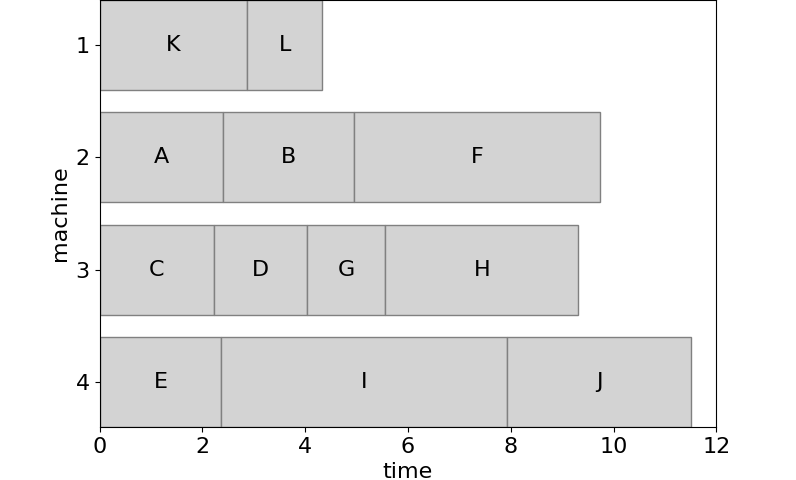
\includegraphics[scale=0.25]{figures/inefficient_makespan.png}};
				\node (right) at (6, 0){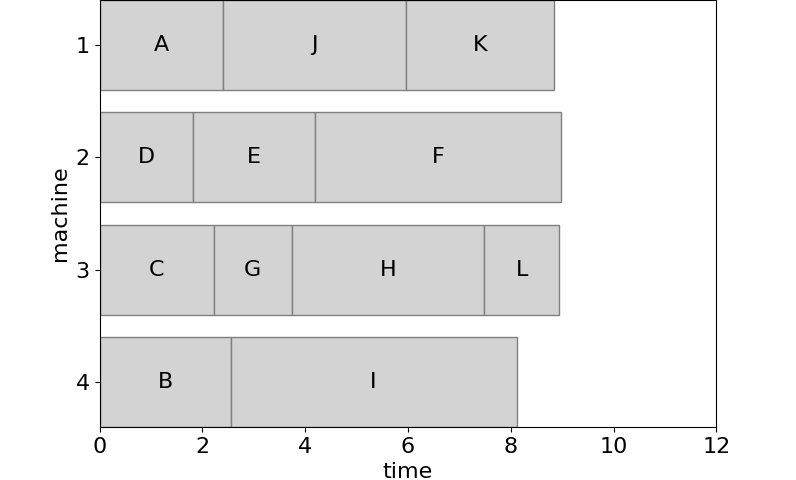
\includegraphics[scale=0.25]{figures/efficient_makespan.png}};
				\draw[thick,->] (left) -- (right) node[midway, above] {optimise};
			\end{tikzpicture}
		}
		\begin{itemize}
			\item Solvers and schedules are difficult to understand
			\item Apply argumentation to makespan schedules to generate explanations
		\end{itemize}
	\end{frame}

	\begin{frame}
		\frametitle{Contributions}
		\begin{columns}
			\begin{column}{0.5\textwidth}
				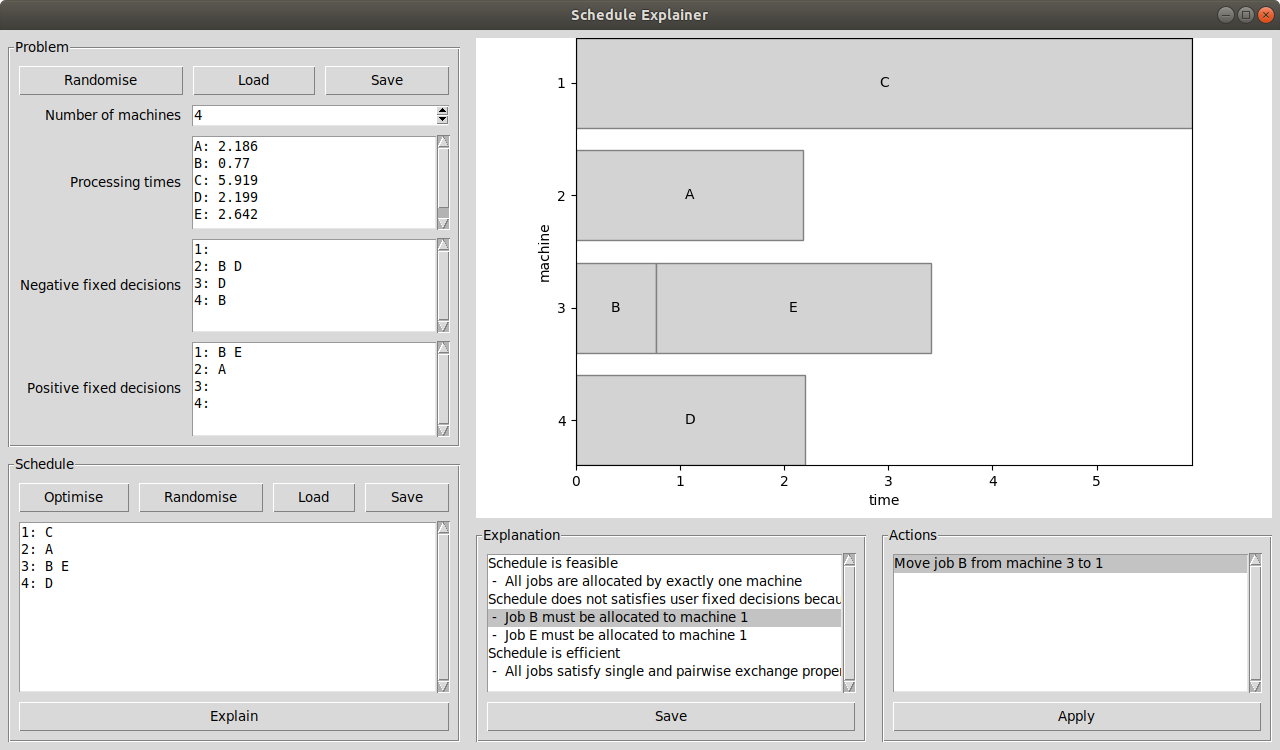
\includegraphics[width=\textwidth]{figures/tool_gui.png}
			\end{column}
			\begin{column}{0.5\textwidth}
				\resizebox{\textwidth}{!}{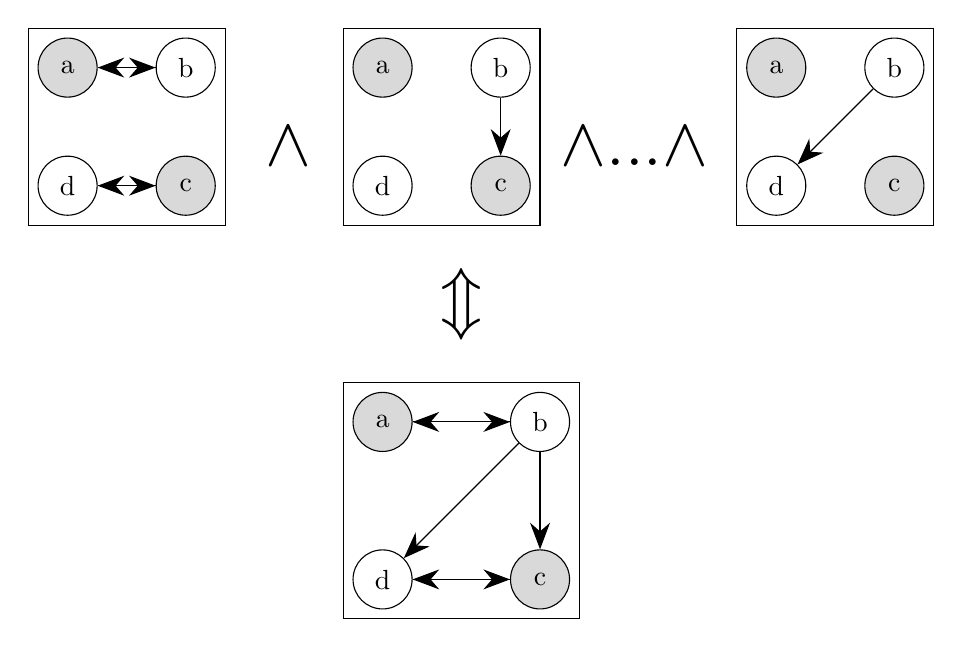
\begin{tikzpicture}
	\node[node, shaded](a) at (0, 1.5){a};
	\node[node](b) at (1.5, 1.5){b};
	\node[node, shaded](c) at (1.5, 0){c};
	\node[node](d) at (0, 0){d};
	\draw[arrow](a) -- (b);
	\draw[arrow](b) -- (a);
	\draw[arrow](c) -- (d);
	\draw[arrow](d) -- (c);
	\draw(-0.5,-0.5) rectangle (2,2);
	\node at (2.8, 0.5){\Huge{$\land$}};

	\node[node, shaded](a) at (4, 1.5){a};
	\node[node](b) at (5.5, 1.5){b};
	\node[node, shaded](c) at (5.5, 0){c};
	\node[node](d) at (4, 0){d};
	\draw[arrow](b) -- (c);
	\draw(3.5,-0.5) rectangle (6,2);
	\node at (7.2, 0.5){\Huge{$\land...\land$}};

	\node[node, shaded](a) at (9, 1.5){a};
	\node[node](b) at (10.5, 1.5){b};
	\node[node, shaded](c) at (10.5, 0){c};
	\node[node](d) at (9, 0){d};
	\draw[arrow](b) -- (d);
	\draw(8.5,-0.5) rectangle (11,2);
	\node at (5, -1.5){\Huge{$\Updownarrow$}};

	\node[node, shaded](a) at (4, -3){a};
	\node[node](b) at (6, -3){b};
	\node[node, shaded](c) at (6, -5){c};
	\node[node](d) at (4, -5){d};
	\draw[arrow](a) -- (b);
	\draw[arrow](b) -- (a);
	\draw[arrow](b) -- (c);
	\draw[arrow](b) -- (d);
	\draw[arrow](c) -- (d);
	\draw[arrow](d) -- (c);
	\draw(3.5,-5.5) rectangle (6.5, -2.5);
\end{tikzpicture}}
			\end{column}
		\end{columns}

		\begin{columns}
			\begin{column}{0.5\textwidth}
				\begin{itemize}
					\item Interactive tool
					\item Algorithms
				\end{itemize}
			\end{column}
			\begin{column}{0.5\textwidth}
				\begin{itemize}
					\item Theoretical extensions 
					\item Discussion
				\end{itemize}
			\end{column}
		\end{columns}			
	\end{frame}

	\begin{frame}
		\frametitle{Demonstration}
		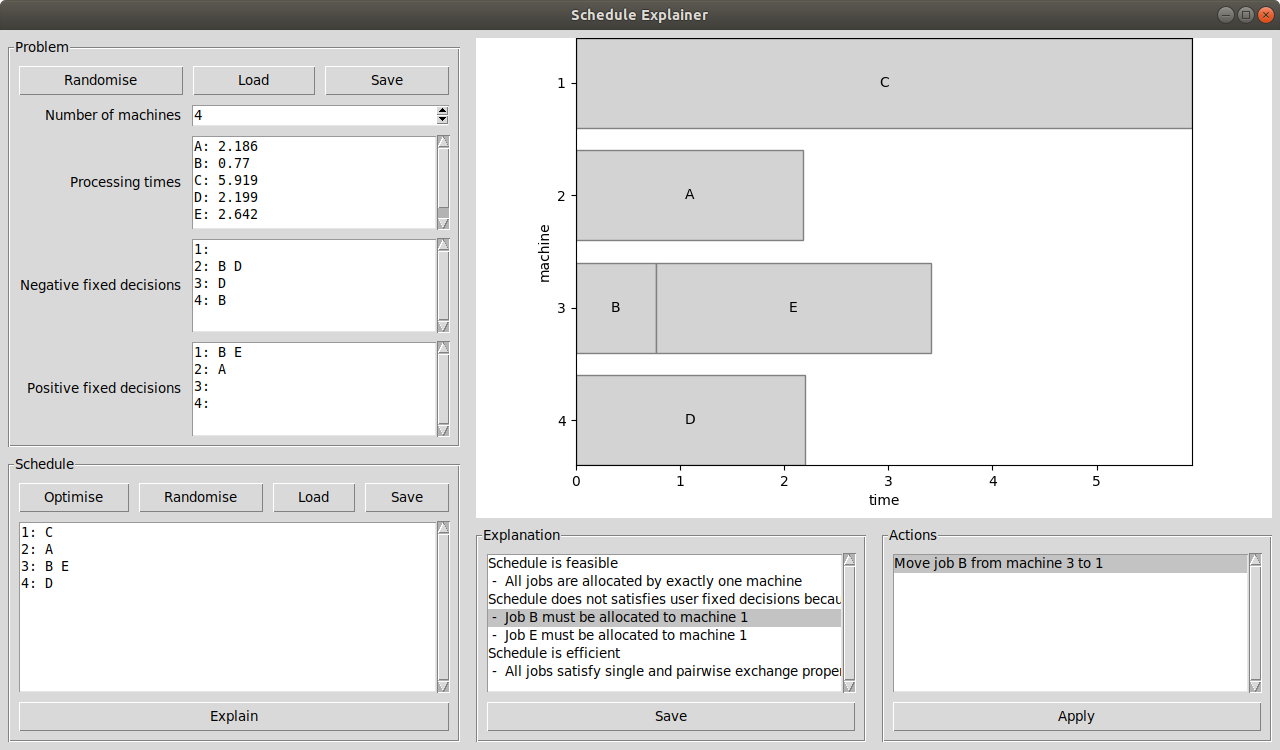
\includegraphics[width=\textwidth]{figures/tool_gui.png}
	\end{frame}

	\subsection{Interactive Tool and Algorithms}

	\begin{frame}
		\frametitle{Abstract Argumentation}
		\begin{itemize}
			\item An abstract argumentation framework is a directed graph $\pair{Args}{\rightsquigarrow}$.
			\item Extension $E$ is a subset of $Args$.
		\end{itemize}
		
		\begin{definition}
			$E$ is conflict-free on $\pair{Args}{\rightsquigarrow}$ iff $\forall a,b\in E. a\not\rightsquigarrow b$.
		\end{definition}
	
		\begin{definition}
			$E$ is stable on $\pair{Args}{\rightsquigarrow}$ iff $E$ is conflict-free on $\pair{Args}{\rightsquigarrow}$ and $\forall a\in Args\setminus E.\exists e\in E.e\rightsquigarrow a$.
		\end{definition}
	\end{frame}

	\begin{frame}[label=pipeline]
		\frametitle{Pipeline}
		\resizebox{\textwidth}{!}{\begin{tikzpicture}
	\node[draw, align=center] (problem) at (0, 3){$m=2$\\$n=3$\\$\mathbf{p}=[2,4,5]$\\$D=\varnothing$};

	\draw(2,2) rectangle (4, 4);
	\node[draw, circle] (a) at (2.5, 2.5){};
	\node[draw, circle] (b) at (3, 2.5){};
	\node[draw, circle] (c) at (3.5, 2.5){};
	\node[draw, circle] (d) at (2.5, 3.5){};
	\node[draw, circle] (e) at (3, 3.5){};
	\node[draw, circle] (f) at (3.5, 3.5){};
	\draw[<->] (a) -- (d);
	\draw[<->] (b) -- (e);
	\draw[<->] (c) -- (f);

	\node (chart) at (0, 0){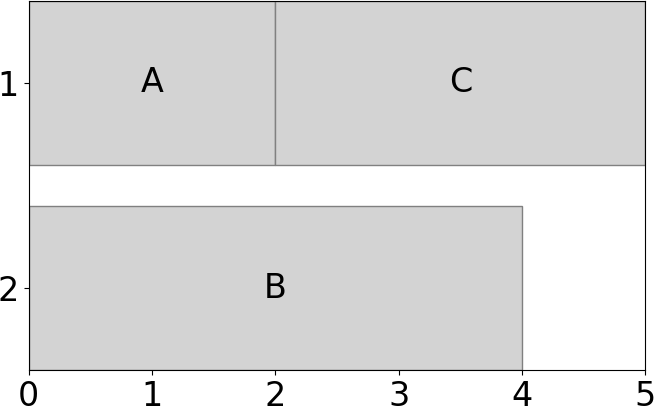
\includegraphics[scale=0.15]{figures/tiny_makespan.png}};
	\node (matrix) at (3, 0){$\begin{bmatrix}
		1 & 0 & 1\\
		0 & 1 & 0\\
		\end{bmatrix}$
	};

	\draw(5,0) rectangle (7, 2);
	\node[draw, circle] (a) at (5.5, 0.5){};
	\node[shaded,draw, circle] (b) at (6, 0.5){};
	\node[draw, circle] (c) at (6.5, 0.5){};
	\node[shaded,draw, circle] (d) at (5.5, 1.5){};
	\node[draw, circle] (e) at (6, 1.5){};
	\node[shaded,draw, circle] (f) at (6.5, 1.5){};
	\draw[<->] (a) -- (d);
	\draw[<->] (b) -- (e);
	\draw[<->] (c) -- (f);
	
	\node[draw](text) at (9, 1){Explanation};
	
	\draw[arrow] (problem) -- (2, 3);
	\draw[arrow, dashed] (problem) -- (chart);
	\draw[arrow] (4, 2.333) -- (5, 1.666);
	\draw[arrow] (chart) -- (matrix);
	\draw[arrow] (matrix) -- (5, 0.666);
	\draw[arrow] (7, 1) -- (text);
\end{tikzpicture}}
	\end{frame}

	\begin{frame}
		\frametitle{Feasibility Framework Construction}
				
		\begin{columns}
			\begin{column}{0.5\textwidth}
				\begin{center}
					$\begin{bmatrix}
						1 & 0 & 1\\
						0 & 1 & 0\\
					\end{bmatrix}$
					\begin{equation*}
						\forall j\in\mathcal{J}.\sum_{i\in\mathcal{M}}x_{i,j}=1
					\end{equation*}
				\end{center}
			\end{column}
			\begin{column}{0.5\textwidth}
				\begin{center}
					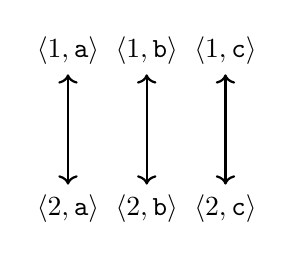
\begin{tikzpicture}
						\node(a) at (0, 0){$\pair{2}{\mathtt{a}}$};
						\node(b) at (1, 0){$\pair{2}{\mathtt{b}}$};
						\node(c) at (2, 0){$\pair{2}{\mathtt{c}}$};
						\node(d) at (0, 2){$\pair{1}{\mathtt{a}}$};
						\node(e) at (1, 2){$\pair{1}{\mathtt{b}}$};
						\node(f) at (2, 2){$\pair{1}{\mathtt{c}}$};
						
						\draw[thick,<->](a) -- (d);
						\draw[thick,<->](b) -- (e);
						\draw[thick,<->](c) -- (f);
					\end{tikzpicture}
					$Args_F=\mathcal{M}\times\mathcal{J}$\\
					$\pair{i}{j}\rightsquigarrow_F\pair{i'}{j'}$ iff $i\neq i'\land j=j'$
				\end{center}
			\end{column}
		\end{columns}
	\end{frame}

	\begin{frame}
		\frametitle{Framework Modelling}
		
		\begin{definition}
			Framework $\pair{Args}{\rightsquigarrow}$ stability-models a property $P$ iff $\forall E\subseteq Args.E$ is stable on $\pair{Args}{\rightsquigarrow}\Leftrightarrow P$
		\end{definition}
	
		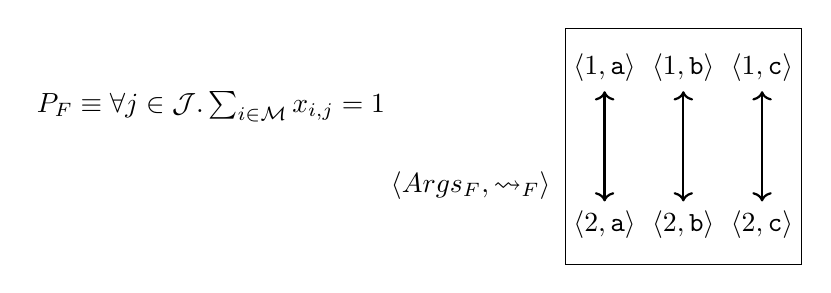
\begin{tikzpicture}
			\node(a) at (0, 0){$\pair{2}{\mathtt{a}}$};
			\node(b) at (1, 0){$\pair{2}{\mathtt{b}}$};
			\node(c) at (2, 0){$\pair{2}{\mathtt{c}}$};
			\node(d) at (0, 2){$\pair{1}{\mathtt{a}}$};
			\node(e) at (1, 2){$\pair{1}{\mathtt{b}}$};
			\node(f) at (2, 2){$\pair{1}{\mathtt{c}}$};
			
			\draw[thick,<->](a) -- (d);
			\draw[thick,<->](b) -- (e);
			\draw[thick,<->](c) -- (f);
			
			\node at (-1.7, 0.5){$\pair{Args_F}{\rightsquigarrow_F}$};
			\draw (-0.5, -0.5) rectangle (2.5, 2.5);
			
			\node at (-5, 1.5){$P_F\equiv\forall j\in\mathcal{J}.\sum_{i\in\mathcal{M}}x_{i,j}=1$};
		\end{tikzpicture}
		
		\begin{theorem}
			$\pair{Args_F}{\rightsquigarrow_F}$ \textnormal{stability-models} $P_F$
		\end{theorem}
	\end{frame}

	\begin{frame}
		\frametitle{Algorithm Notation}

		\begin{columns}
			\begin{column}{0.5\textwidth}
				\begin{align*}
					\mathbf{0}^{2\times 2}&=
					\begin{bmatrix}
						0&0\\
						0&0\\
					\end{bmatrix}
				\end{align*}

				\begin{align*}
					\begin{bmatrix}
						0&0\\
						1&1\\
					\end{bmatrix}
					\incircbin{\land}
					\begin{bmatrix}
						0&1\\
						0&1\\
					\end{bmatrix}
					&=
					\begin{bmatrix}
						0&0\\
						0&1\\
					\end{bmatrix}
				\end{align*}
			\end{column}
			\begin{column}{0.5\textwidth}		
				\begin{align*}
					\incircbin{\neg}
					\begin{bmatrix}
						1&0\\
						0&1\\
					\end{bmatrix}&=
					\begin{bmatrix}
						0&1\\
						1&0\\
					\end{bmatrix}
				\end{align*}
				
				\begin{align*}
					\begin{bmatrix}
						0&0\\
						1&1\\
					\end{bmatrix}
					\incircbin{\lor}
					\begin{bmatrix}
						0&1\\
						0&1\\
					\end{bmatrix}
					&=
					\begin{bmatrix}
						0&1\\
						1&1\\
					\end{bmatrix}
				\end{align*}
			\end{column}
		\end{columns}		
	\end{frame}

	\begin{frame}
		\frametitle{Construct-Feasibility Algorithm}
		\begin{algorithm}[H]
			\caption{}
			\begin{algorithmic}[1]
				\Function{Construct-Feasibility}{$m$, $n$}
				\State $\twoheadrightarrow_F$ $\gets$ $\mathbf{0}^{(m\times n)^2}$
				\For{$i_1,i_2\in\mathcal{M},j\in\mathcal{J}$}
				\If{$i_1\neq i_2$}
				\State ${\twoheadrightarrow_F}_{i_1,j,i_2,j}$ $\gets$ 1
				\EndIf
				\EndFor
				\State \Return $\twoheadrightarrow_F$
				\EndFunction
			\end{algorithmic}
		\end{algorithm}
	\end{frame}

	\begin{frame}
		\frametitle{Explain-Stability Algorithm}
		\vspace{-0.3\baselineskip}
		\begin{algorithm}[H]
			\caption{}
			\begin{algorithmic}[1]
				\Function{Explain-Stability}{$\mathbf{x}$, $\twoheadrightarrow$, $\bar{\mathbf{u}}$, $\bar{\mathbf{c}}$}
				\State $\mathbf{u}$ $\gets\incircbin{\neg}$ $\mathbf{x}$
				\State $\mathbf{c}$ $\gets\mathbf{0}^{(m\times n)^2}$
				\For{$i\in\mathcal{M},j\in\mathcal{J}$}
				\If{$x_{i,j}=1$}
				\State $\mathbf{u}$ $\gets$ $\mathbf{u}$ $\incircbin{\land}$ $\incircbin{\neg}\twoheadrightarrow_{i,j}$
				\State $c_{i,j}$ $\gets$ $\mathbf{x}$ $\incircbin{\land}$ $\twoheadrightarrow_{i,j}$ 
				\EndIf
				\EndFor			
				\State $\mathbf{u}$ $\gets$ $\mathbf{u}$ $\incircbin{\land}$ $\incircbin{\neg}$ $\bar{\mathbf{u}}$
				\State $\mathbf{c}$ $\gets$ $\mathbf{c}$ $\incircbin{\land}$ $\incircbin{\neg}$ $\bar{\mathbf{c}}$
				\State \Return $\pair{\mathbf{u}}{\mathbf{c}}$
				\EndFunction
			\end{algorithmic}
		\end{algorithm}
	\end{frame}

	\begin{frame}
		\frametitle{Explain-Feasibility Algorithm}
		\vspace{-0.8\baselineskip}
		\scalebox{0.64}{\begin{minipage}{1.5625\textwidth}
			\begin{algorithm}[H]
				\caption{}
				\begin{algorithmic}[1]
					\Function{Explain-Feasibility}{$\mathbf{u}$, $\mathbf{c}$}
						\If{$m=0$}
							\If{$n=0$}
								\State \emph{There are no jobs, so the schedule is trivially feasible.}
							\Else
								\State \emph{There are no machines to allocate to jobs.}
							\EndIf
						\Else
							\If{$\mathbf{u}=\mathbf{0}\land\mathbf{c}=\mathbf{0}$}
							\State \emph{All jobs are allocated to exactly one machine.}
							\Else
							\For{$j\in\mathcal{J}$}
							\If{$u_{:,j}=1$}
							\State \emph{Job $j$ is not allocated to any machine.}
							\EndIf
							\If{$c_{:,j,:,j}\neq\mathbf{0}$}
							\State \emph{Job $j$ is over-allocated to machines $\{i\ |\ i\in\mathcal{M}, x_{i,j}=1\}$.}
							\EndIf
							\EndFor
							\EndIf
						\EndIf
					\EndFunction
					\end{algorithmic}
			\end{algorithm}
		\end{minipage}}
	\end{frame}

	\againframe{pipeline}

	\begin{frame}
		\frametitle{Algorithms Overview}
		\begin{center}
			\resizebox{0.9\textwidth}{!}{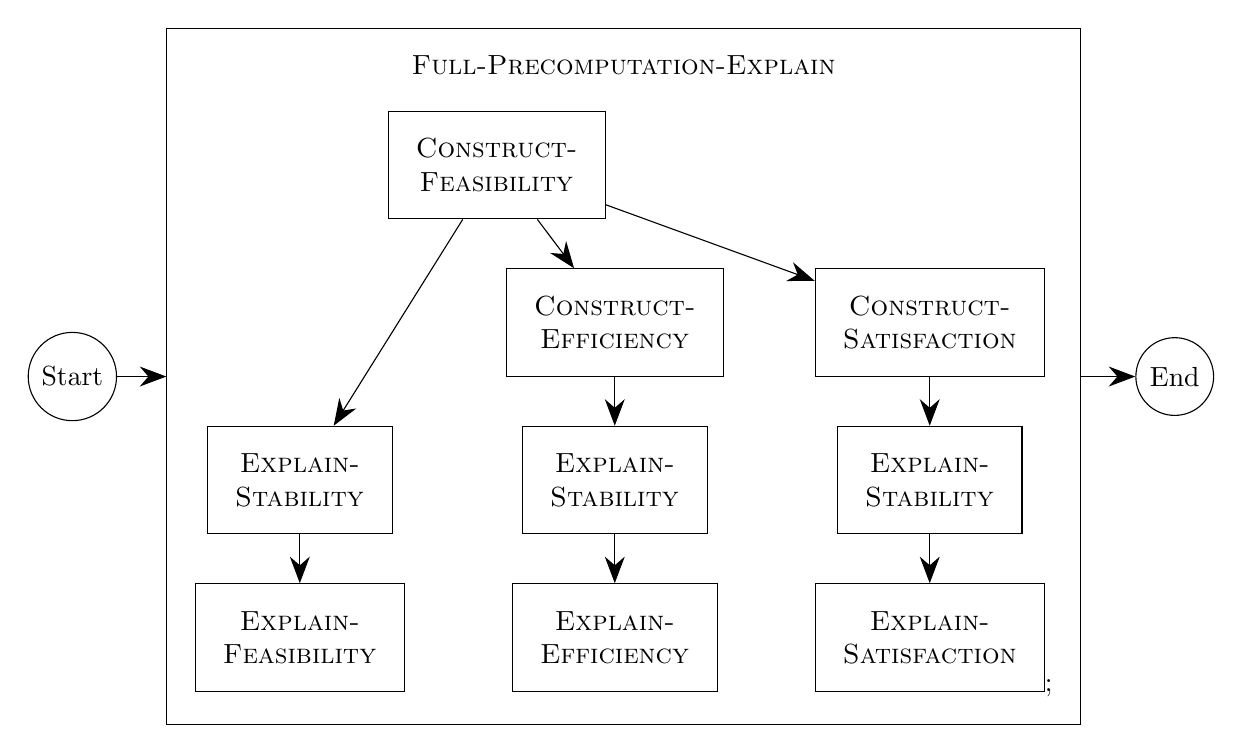
\begin{tikzpicture}
	\node[node](start) at (-7, 6){Start};
	\node[file, align=center](fpe) at (0, 6){
		\textsc{Full-Precomputation-Explain}
		\\\\
		\tikz{
			\node[file](cf) at (2.5, 8){\textsc{Construct-}\\\textsc{Feasibility}};
			\node[file](ce) at (4, 6){\textsc{Construct-}\\\textsc{Efficiency}};
			\node[file](cs) at (8, 6){\textsc{Construct-}\\\textsc{Satisfaction}};
			\node[file](sf) at (0, 4){\textsc{Explain-}\\\textsc{Stability}};
			\node[file](se) at (4, 4){\textsc{Explain-}\\\textsc{Stability}};
			\node[file](ss) at (8, 4){\textsc{Explain-}\\\textsc{Stability}};
			\node[file](ef) at (0, 2){\textsc{Explain-}\\\textsc{Feasibility}};
			\node[file](ee) at (4, 2){\textsc{Explain-}\\\textsc{Efficiency}};
			\node[file](es) at (8, 2){\textsc{Explain-}\\\textsc{Satisfaction}};
			\draw[arrow](cf) -- (sf);
			\draw[arrow](cf) -- (ce);
			\draw[arrow](cf) -- (cs);
			\draw[arrow](ce) -- (se);
			\draw[arrow](cs) -- (ss);
			\draw[arrow](sf) -- (ef);
			\draw[arrow](se) -- (ee);
			\draw[arrow](ss) -- (es);
		};
	};
	\node[node](end) at (7, 6){End};
	\draw[arrow](start) -- (fpe);
	\draw[arrow](fpe) -- (end);
\end{tikzpicture}}		
		\end{center}
	\end{frame}

	\begin{frame}
		\frametitle{Generating Efficiency Explanations}
		
		\begin{columns}
			\begin{column}{0.5\textwidth}
						\begin{itemize}
					\item Single and pair-wise exchange properties
					\item Fixed decision awareness
					\item Explanations are:
					\begin{itemize}
						\item superfluous
						\item local
						\item expensive
					\end{itemize}
				\end{itemize}
			\end{column}
			\begin{column}{0.5\textwidth}
				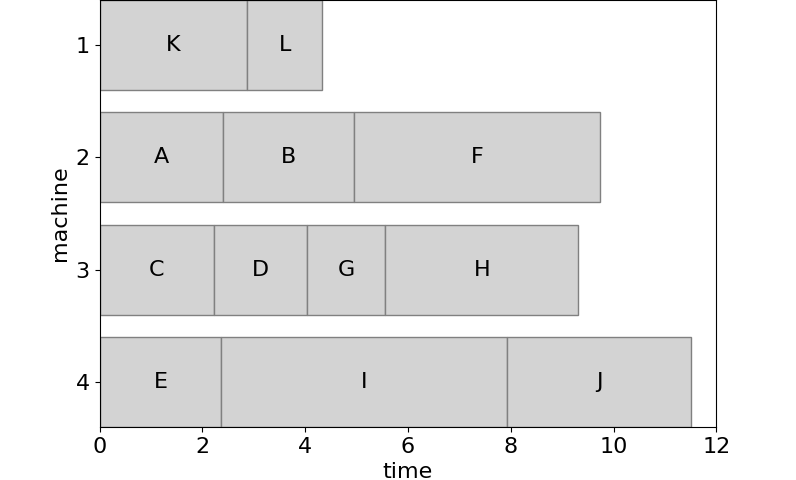
\includegraphics[width=\textwidth]{figures/inefficient_makespan.png}
			\end{column}
		\end{columns}
	\end{frame}

	\begin{frame}
		\frametitle{Generating Fixed Decisions Explanations}
		\scalebox{0.8}{\begin{minipage}{1.125\textwidth}
			\begin{algorithm}[H]
				\caption{}
				\begin{algorithmic}[1]
					\Function{Explain-Satisfaction}{$D$, $\mathbf{u}$, $\mathbf{c}$}
						\For{$j\in\mathcal{J}$}
							\If{$\exists i\in\mathcal{M}\ \pair{i}{j}\not\in D^-$}
								\State\emph{Job $j$ cannot be allocated to any machine.}
							\EndIf
							\If{$D^-$ and $D^+$ are not disjoint}
								\State\emph{Job $j$ has conflicting negative and positive fixed decisions.}
							\EndIf
							\If{$|\{i\in\mathcal{M}\ |\ \pair{i}{j}\in D^+\}|>1$}
								\State\emph{Job $j$ cannot be allocated to multiple machines.}	
							\EndIf
						\EndFor
						\State ...
					\EndFunction
				\end{algorithmic}
			\end{algorithm}		
		\end{minipage}}
	\end{frame}

	\begin{frame}
		\frametitle{Partial-Precomputation Optimisation}
		\begin{itemize}
			\item $\twoheadrightarrow$ construction has $\mathcal{O}(m^2n^2)$ memory usage.
			\item Inline stability and framework construction algorithms
			\item Operate on sub-graphs $\twoheadrightarrow_{i,j}$
		\end{itemize}
		\vspace{\baselineskip}
		\begin{itemize}
			\item Full-Precomputation complexity: $\mathcal{O}(m^2n^2)$
			\item Partial-Precomputation complexity: $\mathcal{O}(mn^2)$
		\end{itemize}
	\end{frame}	
	\subsection{Theoretical Extensions}

	\begin{frame}
		\frametitle{Time-indexed Interval Scheduling}
		\begin{columns}
			\begin{column}{0.5\textwidth}
				\begin{center}
					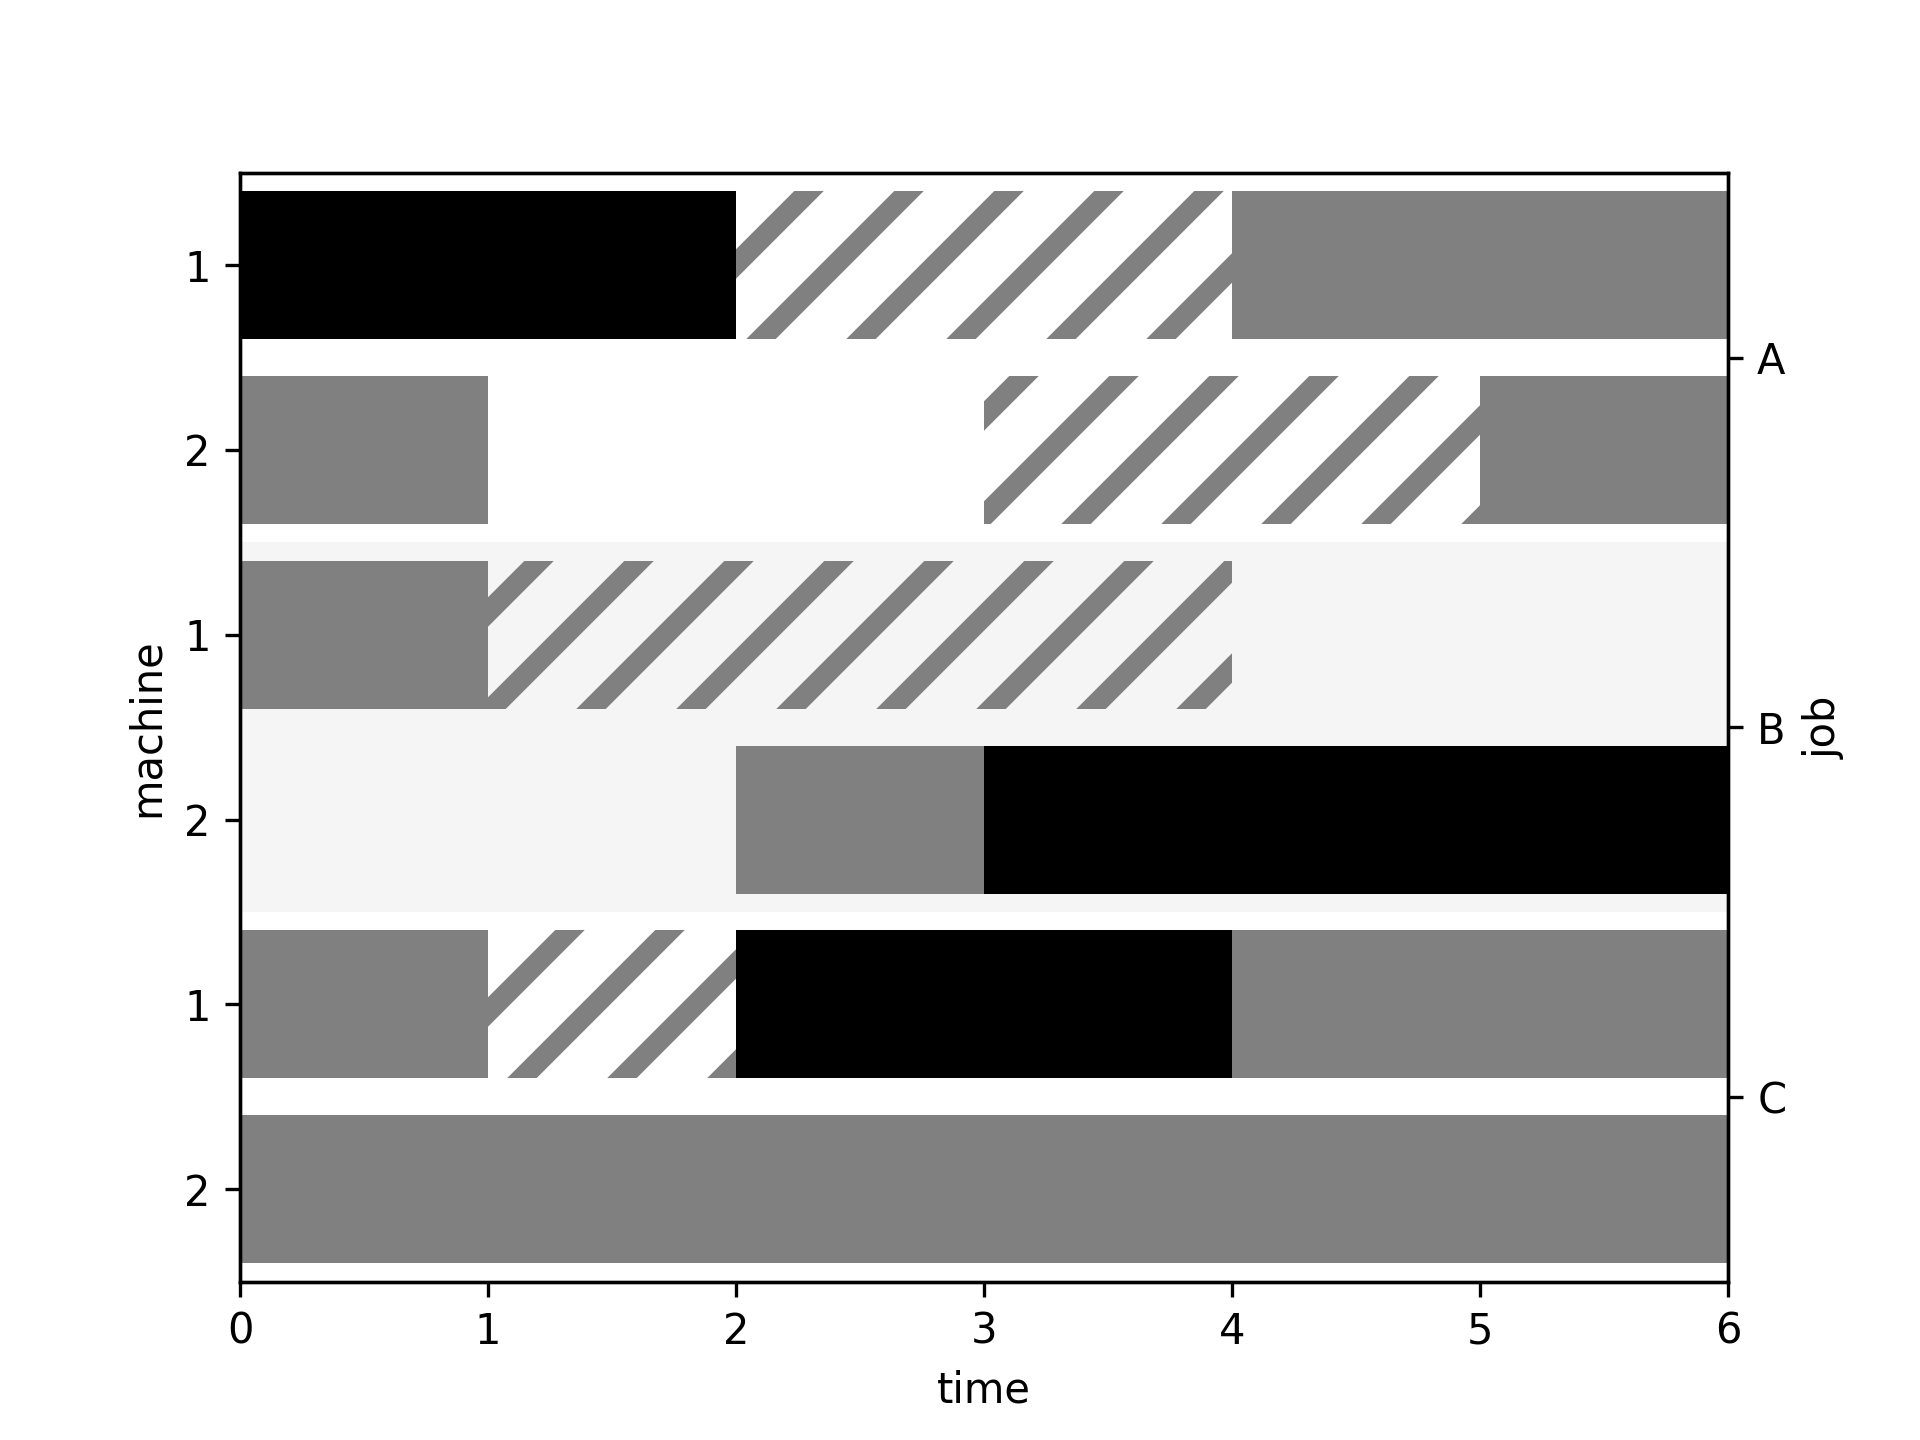
\includegraphics[width=\textwidth]{figures/interval_schedule.png}
				\end{center}
			\end{column}
			\begin{column}{0.5\textwidth}
				\begin{itemize}
					\item Single-allocation of jobs
					\item No overlapping jobs	
					\item Start and finish times
					\item Fixed decisions
				\end{itemize}
			\end{column}
		\end{columns}
	\end{frame}

	\begin{frame}
		\frametitle{Union of Modelling Frameworks Theorem}
		\begin{center}
			\resizebox{0.9\textwidth}{!}{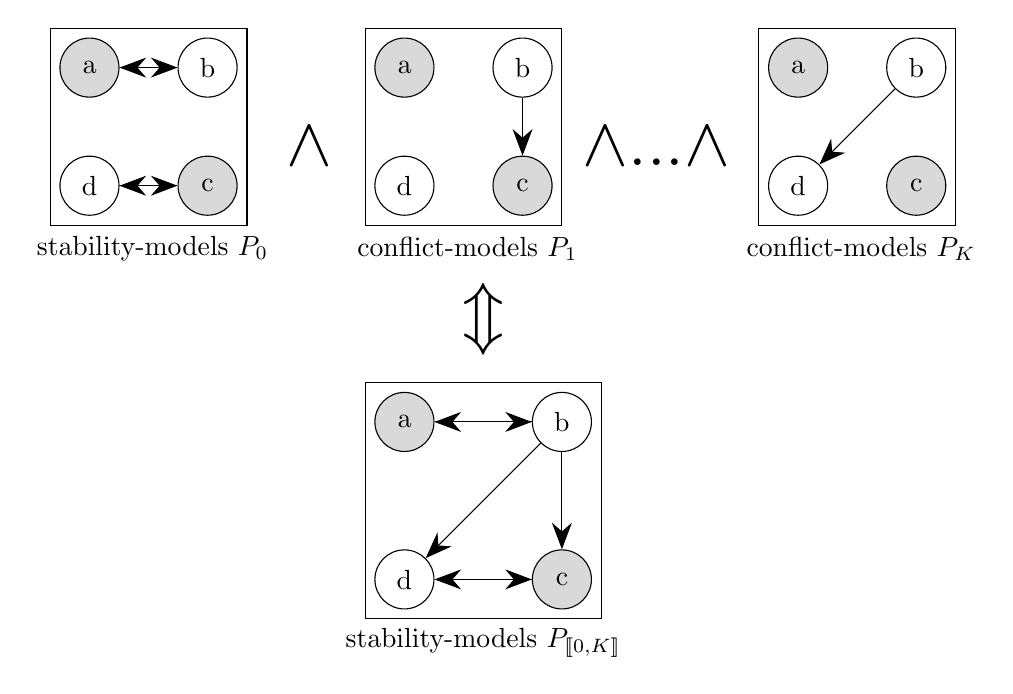
\begin{tikzpicture}
	\node[node, shaded](a) at (0, 1.5){a};
	\node[node](b) at (1.5, 1.5){b};
	\node[node, shaded](c) at (1.5, 0){c};
	\node[node](d) at (0, 0){d};
	\draw[arrow](a) -- (b);
	\draw[arrow](b) -- (a);
	\draw[arrow](c) -- (d);
	\draw[arrow](d) -- (c);
	\draw(-0.5,-0.5) rectangle (2,2);
	\node at (0.8, -0.8){stability-models $P_0$};

	\node at (2.8, 0.5){\Huge{$\land$}};

	\node[node, shaded](a) at (4, 1.5){a};
	\node[node](b) at (5.5, 1.5){b};
	\node[node, shaded](c) at (5.5, 0){c};
	\node[node](d) at (4, 0){d};
	\draw[arrow](b) -- (c);
	\draw(3.5,-0.5) rectangle (6,2);
	\node at (4.8, -0.8){conflict-models $P_1$};

	\node at (7.2, 0.5){\Huge{$\land...\land$}};

	\node[node, shaded](a) at (9, 1.5){a};
	\node[node](b) at (10.5, 1.5){b};
	\node[node, shaded](c) at (10.5, 0){c};
	\node[node](d) at (9, 0){d};
	\draw[arrow](b) -- (d);
	\draw(8.5,-0.5) rectangle (11,2);
	\node at (9.8, -0.8){conflict-models $P_K$};

	\node at (5, -1.7){\Huge{$\Updownarrow$}};

	\node[node, shaded](a) at (4, -3){a};
	\node[node](b) at (6, -3){b};
	\node[node, shaded](c) at (6, -5){c};
	\node[node](d) at (4, -5){d};
	\draw[arrow](a) -- (b);
	\draw[arrow](b) -- (a);
	\draw[arrow](b) -- (c);
	\draw[arrow](b) -- (d);
	\draw[arrow](c) -- (d);
	\draw[arrow](d) -- (c);
	\draw(3.5,-5.5) rectangle (6.5, -2.5);
	\node at (5, -5.8){stability-models $P_{\intset{0,K}}$};
\end{tikzpicture}}		
		\end{center}
	\end{frame}

	\begin{frame}
		\frametitle{Theoretical Applications}
		\begin{definition}
			Property $P$ is stability-modellable iff $\exists\pair{Args}{\rightsquigarrow}.\pair{Args}{\rightsquigarrow}$ stability models $P$.
		\end{definition}
		\begin{theorem}
			\textnormal{Interval scheduling feasibility is stability-modellable.}
		\end{theorem}
	\end{frame}

	\subsection{Evaluation}

	\begin{frame}
		\frametitle{Questionnaire}
		\begin{columns}
			\begin{column}{0.5\textwidth}
				\begin{center}
					\fbox{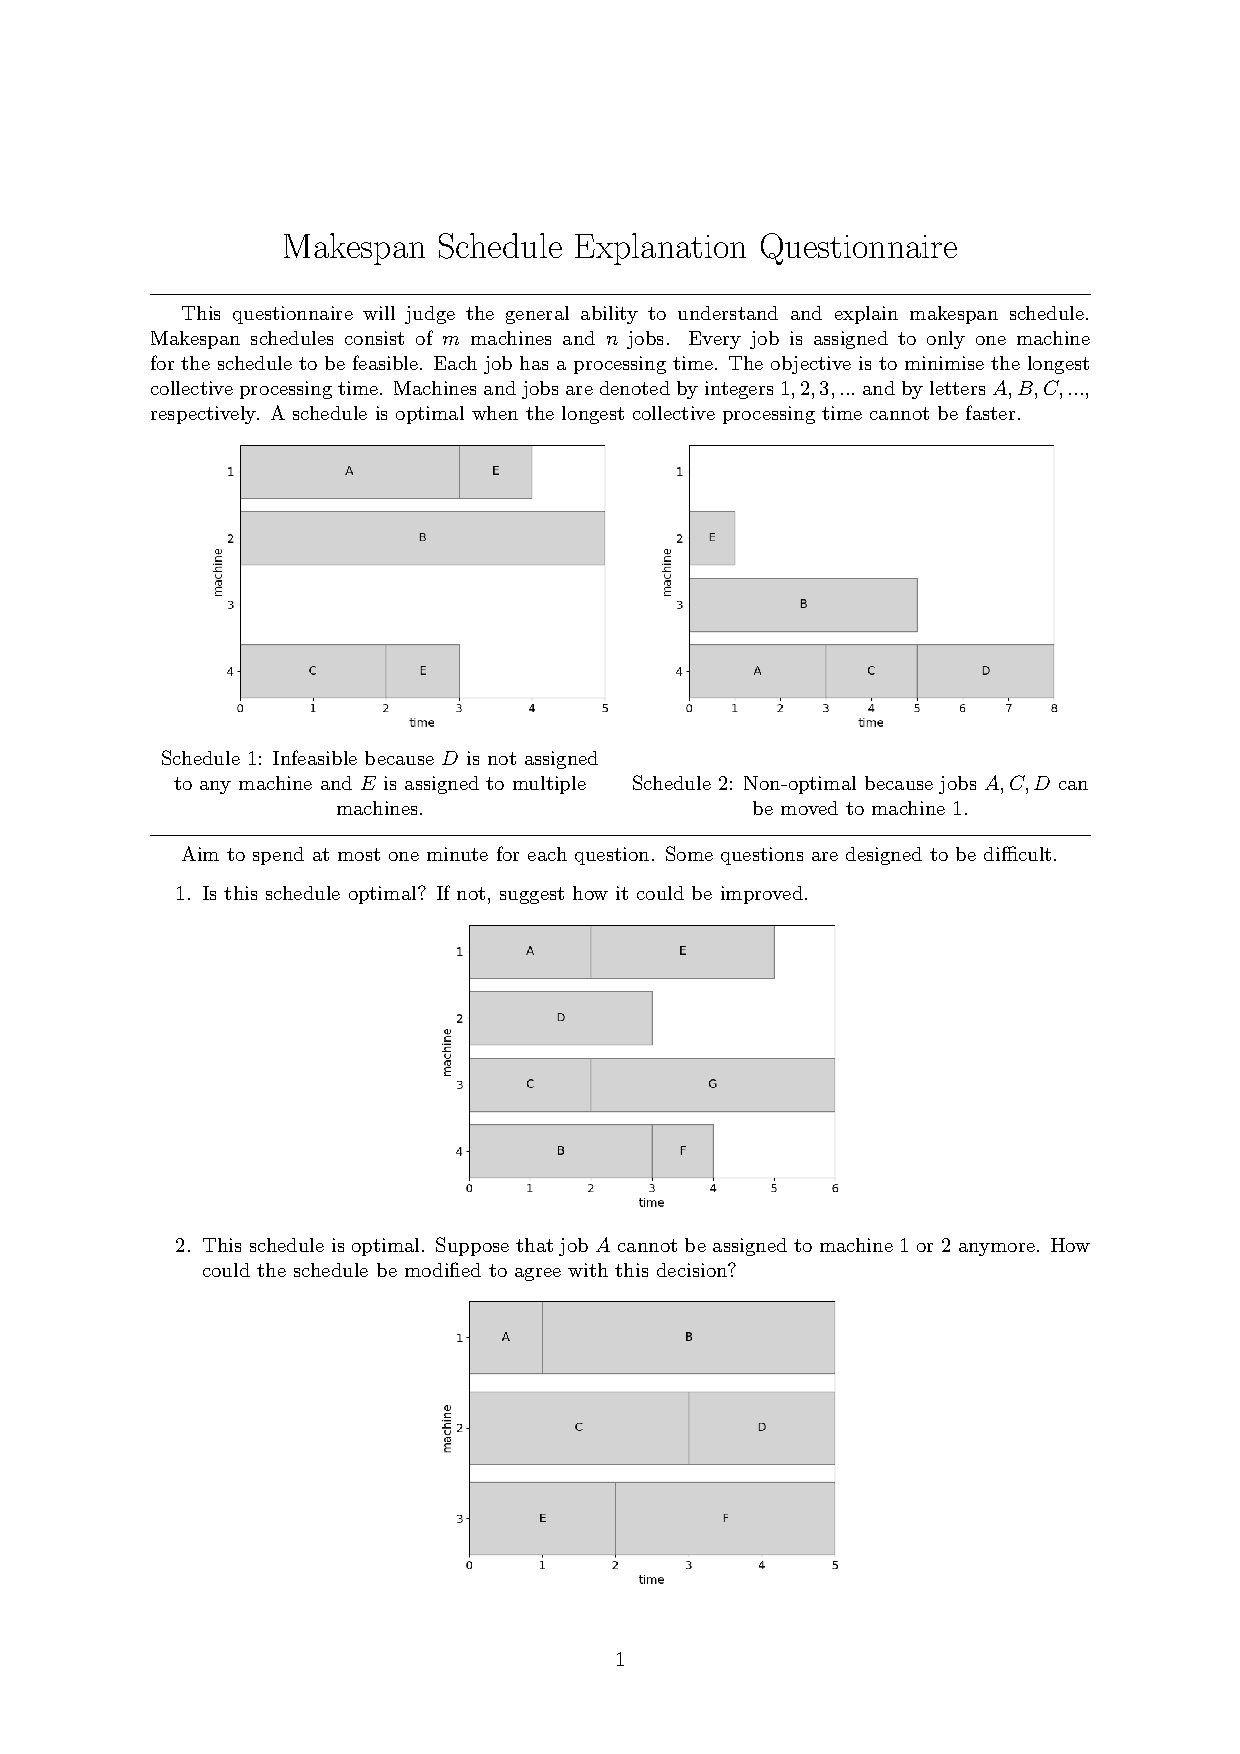
\includegraphics[scale=0.2,page=1]{../report/questionnaire.pdf}}
				\end{center}
			\end{column}
			\begin{column}{0.5\textwidth}
				\begin{center}
					\fbox{\includegraphics[scale=0.2,page=2]{../report/questionnaire.pdf}}
				\end{center}
			\end{column}
		\end{columns}
	\end{frame}

	\begin{frame}
		\frametitle{Questionnaire Results}
		\begin{center}
			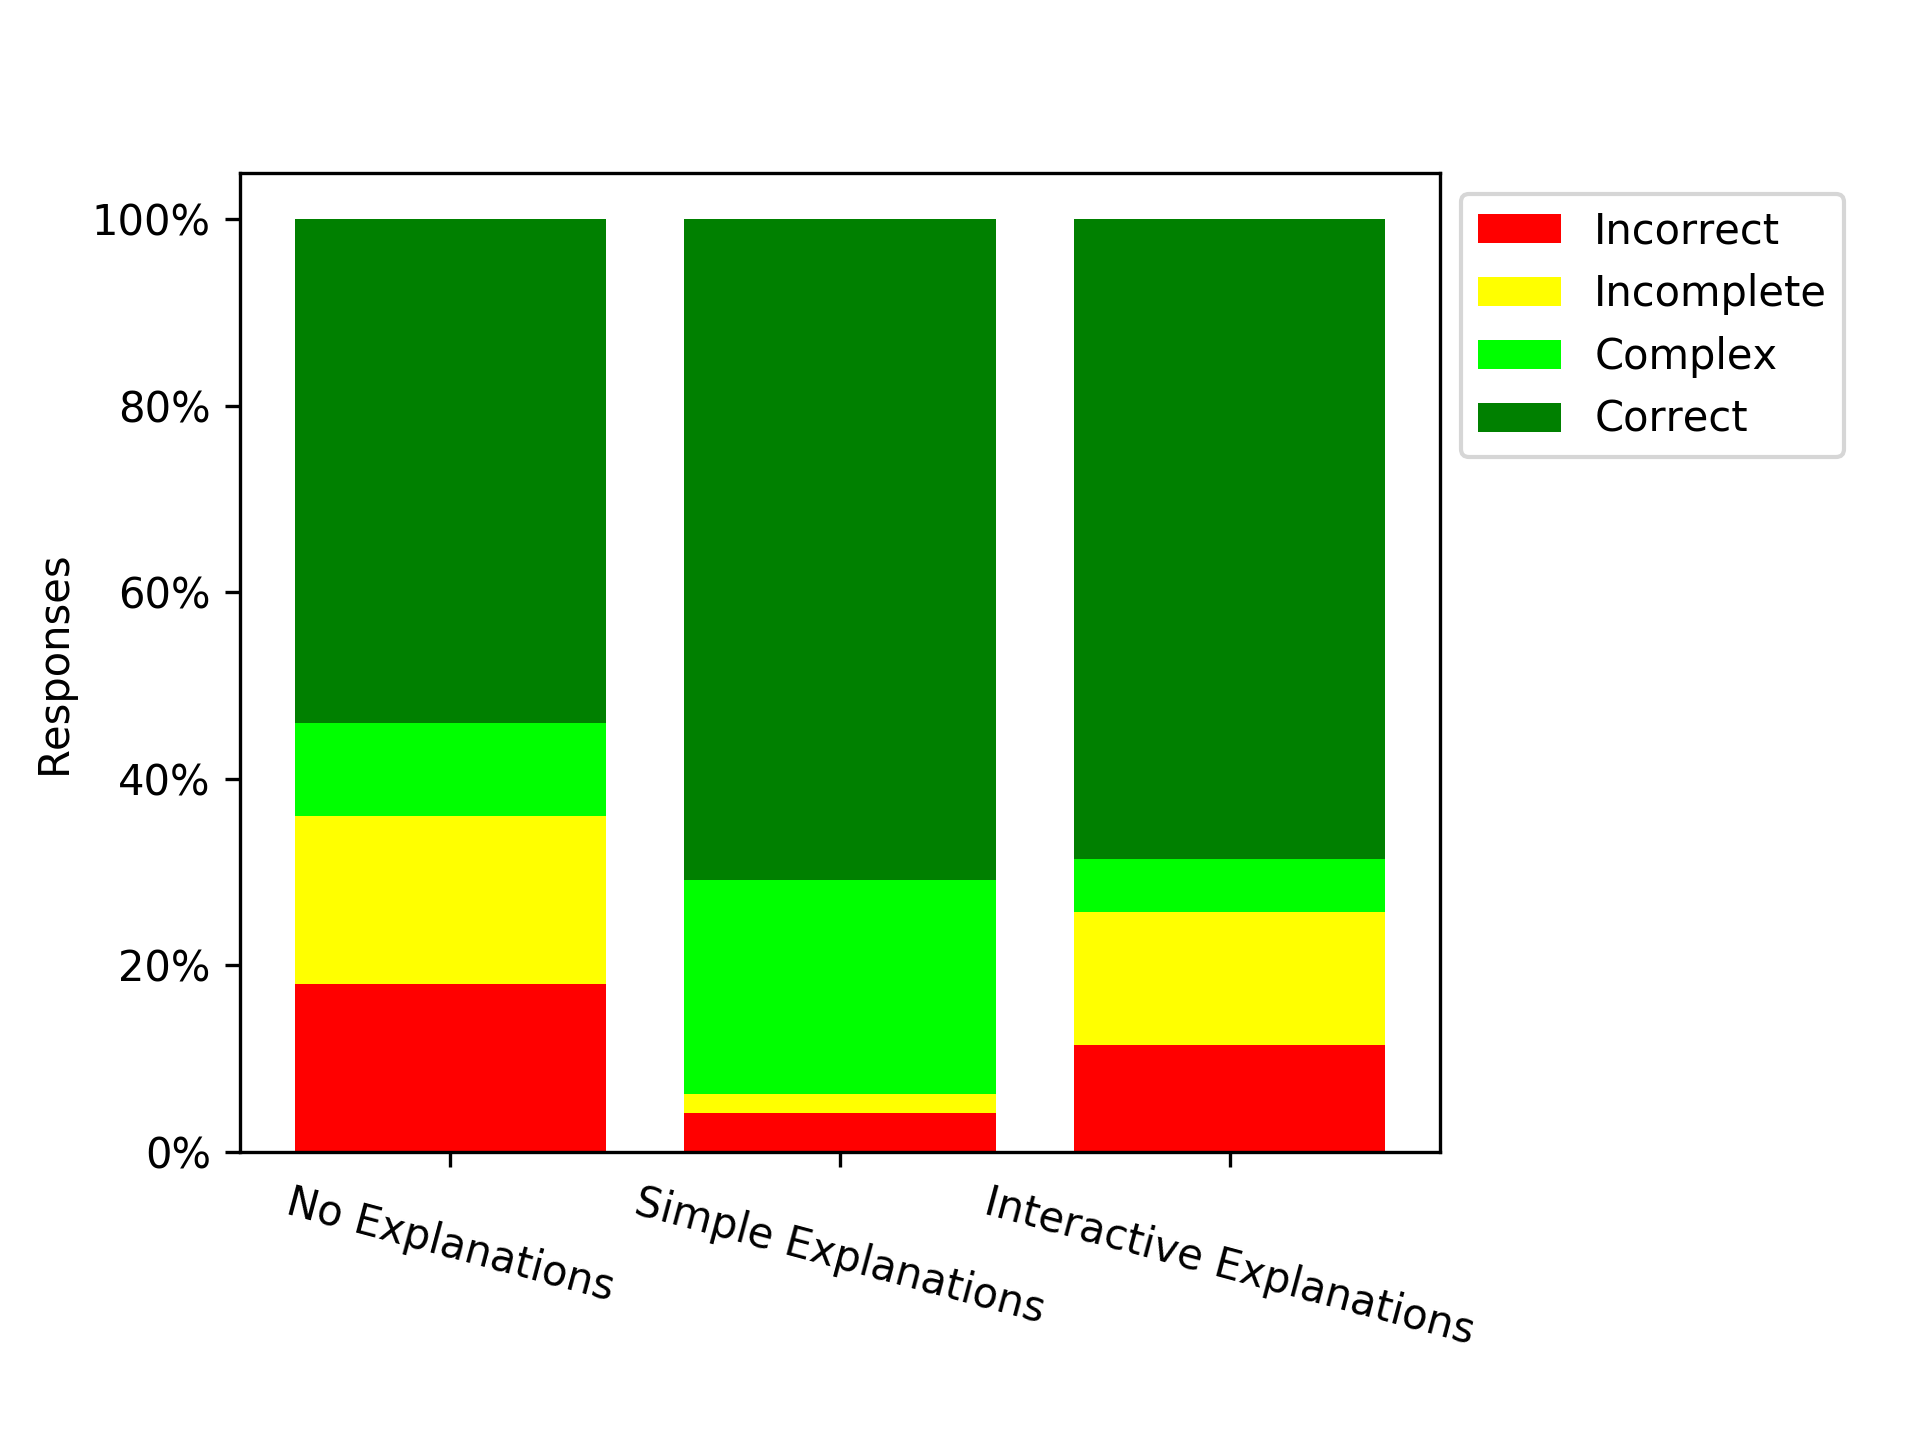
\includegraphics[width=0.8\textwidth]{figures/questionnaire_results_summary.png}
		\end{center}
	\end{frame}

	\begin{frame}
		\frametitle{Profiling}
		\begin{itemize}
			\item $m=10$
		\end{itemize}
		\begin{columns}
			\begin{column}{0.5\textwidth}
				\begin{center}
					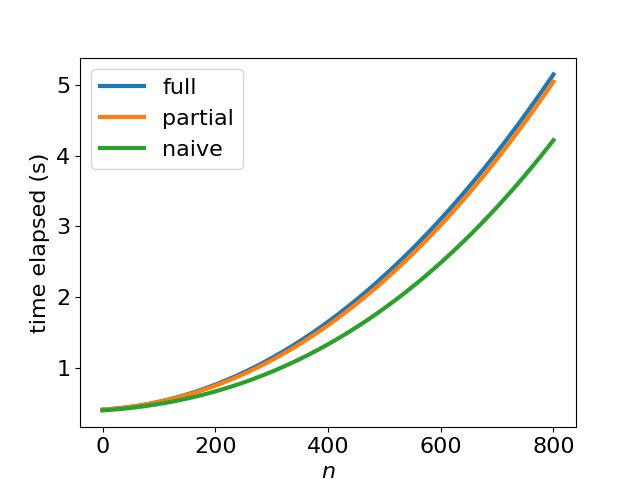
\includegraphics[width=\textwidth]{figures/cpu_profile.png}
					CPU Performance
				\end{center}
			\end{column}
			\begin{column}{0.5\textwidth}
				\begin{center}
					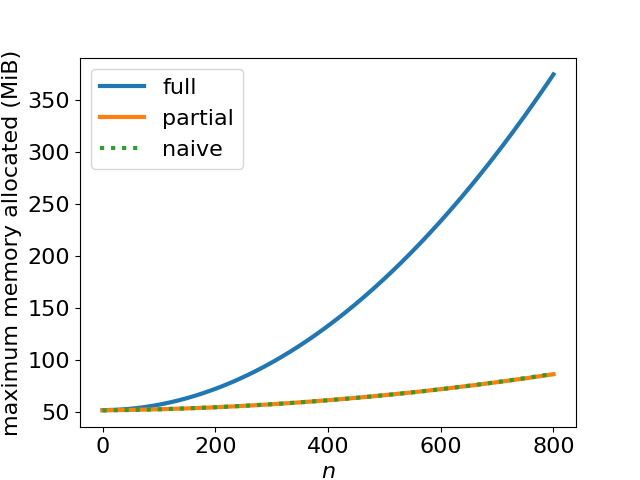
\includegraphics[width=\textwidth]{figures/memory_profile.png}
					Memory Performance
				\end{center}
			\end{column}
		\end{columns}
	\end{frame}

	\subsection{Conclusion}
	\begin{frame}
		blah
	\end{frame}
\end{document}